\documentclass[a4paper,10pt]{article}
\input{/Users/benjamin/Documents/Education/LaTeX/macro.tex}

\title{AEV: S�ance 8}
\author{Benjamin \bsc{Van Ryseghem}}

\begin{document}
\maketitle

\section{Exercice 1: Performances}
\subsection{Question 1}
\[1024 \times 2 + 2\times\dfrac{1024\times1025}{2} = 1024\times 1027 \]

\subsection{Question 2}
Le dernier processeur est celui qui ex�cutera les derni�res instructions (de 993\footnote{1024-32+1} � 1024).

\begin{eqnarray*}
\displaystyle\sum^{1024}_{x=993}1 &=& \displaystyle\sum^{1024}_{x=0}1 - \displaystyle\sum^{992}_{x=0}1 \\
\displaystyle\sum^{1024}_{x=993}1 &=& \dfrac{1024\times1025}{2} - \dfrac{992\times993}{2} \\
\end{eqnarray*}

Facteur d'acc�l�ration: \[ 2\times\dfrac{1024\times 1027}{1024\times1025 - 992\times993}. \]

\subsection{Question 3}
C'est pareil.

\subsection{Question 4}
Il faut distribue en zig-zag.

\begin{tabular}{|c|c|c|c|c|}
\hline
$p_1$ & $p_2$& \dots &$p_31$&$p_32$\\
\hline
1&2&\dots&31&32\\
64&63&\dots&34&33\\
65&66&\dots&95&96\\
\multicolumn{5}{|c|}{\dots}\\
\hline
\end{tabular}

\subsection{Question 5}
Le temps d'ex�cution si l'algorithme est bien �quilibr� est le temps s�quentiel divis� par le nombre de processeurs.

Le facteur d'acc�l�ration est �gal au nombre de processeurs.

\section{Exercice 2}

\begin{figure}[ht]
\begin{center}
     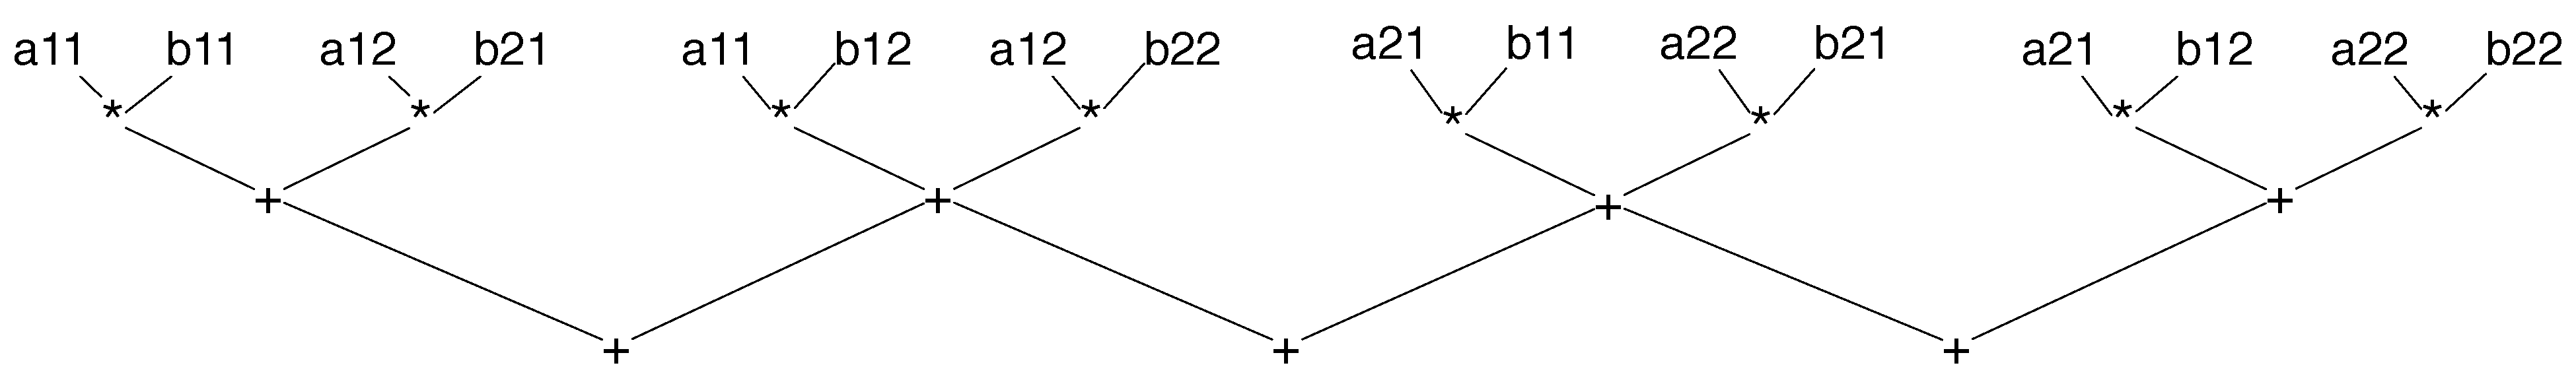
\includegraphics[width=15cm]{figures/exo2}
\end{center}
     \caption{Graphe de multiplication de deux matrices [2x2]}
\end{figure}

\subsection{Question 2}
\paragraph{S�quentiel}
\[ 8 \times 101 + 7 \times 8 = 864 \]
\paragraph{8 processeurs} 761

?
\paragraph{4 processeurs} 650

?
\paragraph{2 processeurs} 
\[ 212+ 4 \times 8+4 \times101 = 648\]

\section{Exercice 3}
\subsection{Question 1}
L'execution d'un programme se d�roule comme suit:
\[ T_{seq} \ T_{seq} \ T_{seq} \ T_{par} \]

De plus, 1 $A$ est execute par $T_{seq}$, quand 9 $A$ sont ex�cut�s par $T_{par}$.
En tout, sur 12 A, 9A sont ex�cut�s en parall�le, soit 75\%.

De plus, en instaurant du parallelisme, on passe de 12$T$ � 4$T$, soit un speedup de 3.

\subsection{Question 2}

Ici, on passe de 12$T$ � $3,5\ T$, soit un speedup de 3.428571429.

\subsection{Question 3}
D'apr�s la loi d'Amdhal,
\[sup = \dfrac{1}{(1-x)+\dfrac{x}{\mbox{unites\_parallele}}}\],

pour conserver un gain de $\dfrac{24}{7}$, il faut
\begin{eqnarray*}
\dfrac{24}{7} &=& \dfrac{1}{(1-x)+\dfrac{x}{9}}\\
\dfrac{24}{7} &=& \dfrac{1}{\dfrac{9-9x+x}{9}}\\
\dfrac{24}{7} &=& \dfrac{9}{9-8x}\\
24\times (9-8x) &=&7\times 9\\
(24-7)\times 9 &=& (8\times24)x\\
x &=& \dfrac{153}{192}\\
\end{eqnarray*}

\signature

\end{document}